
%% bare_adv.tex
%% V1.4b
%% 2015/08/26
%% by Michael Shell
%% See: 
%% http://www.michaelshell.org/
%% for current contact information.
%%
%% This is a skeleton file demonstrating the advanced use of IEEEtran.cls
%% (requires IEEEtran.cls version 1.8b or later) with an IEEE Computer
%% Society journal paper.
%%
%% Support sites:
%% http://www.michaelshell.org/tex/ieeetran/
%% http://www.ctan.org/pkg/ieeetran
%% and
%% http://www.ieee.org/

%%*************************************************************************
%% Legal Notice:
%% This code is offered as-is without any warranty either expressed or
%% implied; without even the implied warranty of MERCHANTABILITY or
%% FITNESS FOR A PARTICULAR PURPOSE! 
%% User assumes all risk.
%% In no event shall the IEEE or any contributor to this code be liable for
%% any damages or losses, including, but not limited to, incidental,
%% consequential, or any other damages, resulting from the use or misuse
%% of any information contained here.
%%
%% All comments are the opinions of their respective authors and are not
%% necessarily endorsed by the IEEE.
%%
%% This work is distributed under the LaTeX Project Public License (LPPL)
%% ( http://www.latex-project.org/ ) version 1.3, and may be freely used,
%% distributed and modified. A copy of the LPPL, version 1.3, is included
%% in the base LaTeX documentation of all distributions of LaTeX released
%% 2003/12/01 or later.
%% Retain all contribution notices and credits.
%% ** Modified files should be clearly indicated as such, including  **
%% ** renaming them and changing author support contact information. **
%%*************************************************************************


% *** Authors should verify (and, if needed, correct) their LaTeX system  ***
% *** with the testflow diagnostic prior to trusting their LaTeX platform ***
% *** with production work. The IEEE's font choices and paper sizes can   ***
% *** trigger bugs that do not appear when using other class files.       ***                          ***
% The testflow support page is at:
% http://www.michaelshell.org/tex/testflow/


% IEEEtran V1.7 and later provides for these CLASSINPUT macros to allow the
% user to reprogram some IEEEtran.cls defaults if needed. These settings
% override the internal defaults of IEEEtran.cls regardless of which class
% options are used. Do not use these unless you have good reason to do so as
% they can result in nonIEEE compliant documents. User beware. ;)
%
%\newcommand{\CLASSINPUTbaselinestretch}{1.0} % baselinestretch
%\newcommand{\CLASSINPUTinnersidemargin}{1in} % inner side margin
%\newcommand{\CLASSINPUToutersidemargin}{1in} % outer side margin
%\newcommand{\CLASSINPUTtoptextmargin}{1in}   % top text margin
%\newcommand{\CLASSINPUTbottomtextmargin}{1in}% bottom text margin




%
\documentclass[10pt,journal,compsoc]{IEEEtran}
% If IEEEtran.cls has not been installed into the LaTeX system files,
% manually specify the path to it like:
% \documentclass[10pt,journal,compsoc]{../sty/IEEEtran}


% For Computer Society journals, IEEEtran defaults to the use of 
% Palatino/Palladio as is done in IEEE Computer Society journals.
% To go back to Times Roman, you can use this code:
%\renewcommand{\rmdefault}{ptm}\selectfont





% Some very useful LaTeX packages include:
% (uncomment the ones you want to load)



% *** MISC UTILITY PACKAGES ***
\usepackage{fancyvrb,enumerate}
\usepackage[pdftex]{graphicx}
\usepackage{here}
\usepackage{caption}

%
%\usepackage{ifpdf}
% Heiko Oberdiek's ifpdf.sty is very useful if you need conditional
% compilation based on whether the output is pdf or dvi.
% usage:
% \ifpdf
%   % pdf code
% \else
%   % dvi code
% \fi
% The latest version of ifpdf.sty can be obtained from:
% http://www.ctan.org/pkg/ifpdf
% Also, note that IEEEtran.cls V1.7 and later provides a builtin
% \ifCLASSINFOpdf conditional that works the same way.
% When switching from latex to pdflatex and vice-versa, the compiler may
% have to be run twice to clear warning/error messages.




% *** CITATION PACKAGES ***
%
\ifCLASSOPTIONcompsoc
  % The IEEE Computer Society needs nocompress option
  % requires cite.sty v4.0 or later (November 2003)
  \usepackage[nocompress]{cite}
\else
  % normal IEEE
  \usepackage{cite}

\fi
% cite.sty was written by Donald Arseneau
% V1.6 and later of IEEEtran pre-defines the format of the cite.sty package
% \cite{} output to follow that of the IEEE. Loading the cite package will
% result in citation numbers being automatically sorted and properly
% "compressed/ranged". e.g., [1], [9], [2], [7], [5], [6] without using
% cite.sty will become [1], [2], [5]--[7], [9] using cite.sty. cite.sty's
% \cite will automatically add leading space, if needed. Use cite.sty's
% noadjust option (cite.sty V3.8 and later) if you want to turn this off
% such as if a citation ever needs to be enclosed in parenthesis.
% cite.sty is already installed on most LaTeX systems. Be sure and use
% version 5.0 (2009-03-20) and later if using hyperref.sty.
% The latest version can be obtained at:
% http://www.ctan.org/pkg/cite
% The documentation is contained in the cite.sty file itself.
%
% Note that some packages require special options to format as the Computer
% Society requires. In particular, Computer Society  papers do not use
% compressed citation ranges as is done in typical IEEE papers
% (e.g., [1]-[4]). Instead, they list every citation separately in order
% (e.g., [1], [2], [3], [4]). To get the latter we need to load the cite
% package with the nocompress option which is supported by cite.sty v4.0
% and later.





% *** GRAPHICS RELATED PACKAGES ***
%
\ifCLASSINFOpdf
  % \usepackage[pdftex]{graphicx}
  % declare the path(s) where your graphic files are
  % \graphicspath{{../pdf/}{../jpeg/}}
  % and their extensions so you won't have to specify these with
  % every instance of \includegraphics
  % \DeclareGraphicsExtensions{.pdf,.jpeg,.png}
\else
  % or other class option (dvipsone, dvipdf, if not using dvips). graphicx
  % will default to the driver specified in the system graphics.cfg if no
  % driver is specified.
  % \usepackage[dvips]{graphicx}
  % declare the path(s) where your graphic files are
  % \graphicspath{{../eps/}}
  % and their extensions so you won't have to specify these with
  % every instance of \includegraphics
  % \DeclareGraphicsExtensions{.eps}
\fi
% graphicx was written by David Carlisle and Sebastian Rahtz. It is
% required if you want graphics, photos, etc. graphicx.sty is already
% installed on most LaTeX systems. The latest version and documentation
% can be obtained at: 
% http://www.ctan.org/pkg/graphicx
% Another good source of documentation is "Using Imported Graphics in
% LaTeX2e" by Keith Reckdahl which can be found at:
% http://www.ctan.org/pkg/epslatex
%
% latex, and pdflatex in dvi mode, support graphics in encapsulated
% postscript (.eps) format. pdflatex in pdf mode supports graphics
% in .pdf, .jpeg, .png and .mps (metapost) formats. Users should ensure
% that all non-photo figures use a vector format (.eps, .pdf, .mps) and
% not a bitmapped formats (.jpeg, .png). The IEEE frowns on bitmapped formats
% which can result in "jaggedy"/blurry rendering of lines and letters as
% well as large increases in file sizes.
%
% You can find documentation about the pdfTeX application at:
% http://www.tug.org/applications/pdftex





% *** MATH PACKAGES ***
%
%\usepackage{amsmath}
% A popular package from the American Mathematical Society that provides
% many useful and powerful commands for dealing with mathematics.
%
% Note that the amsmath package sets \interdisplaylinepenalty to 10000
% thus preventing page breaks from occurring within multiline equations. Use:
%\interdisplaylinepenalty=2500
% after loading amsmath to restore such page breaks as IEEEtran.cls normally
% does. amsmath.sty is already installed on most LaTeX systems. The latest
% version and documentation can be obtained at:
% http://www.ctan.org/pkg/amsmath





% *** SPECIALIZED LIST PACKAGES ***
%\usepackage{acronym}
% acronym.sty was written by Tobias Oetiker. This package provides tools for
% managing documents with large numbers of acronyms. (You don't *have* to
% use this package - unless you have a lot of acronyms, you may feel that
% such package management of them is bit of an overkill.)
% Do note that the acronym environment (which lists acronyms) will have a
% problem when used under IEEEtran.cls because acronym.sty relies on the
% description list environment - which IEEEtran.cls has customized for
% producing IEEE style lists. A workaround is to declared the longest
% label width via the IEEEtran.cls \IEEEiedlistdecl global control:
%
% \renewcommand{\IEEEiedlistdecl}{\IEEEsetlabelwidth{SONET}}
% \begin{acronym}
%
% \end{acronym}
% \renewcommand{\IEEEiedlistdecl}{\relax}% remember to reset \IEEEiedlistdecl
%
% instead of using the acronym environment's optional argument.
% The latest version and documentation can be obtained at:
% http://www.ctan.org/pkg/acronym


%\usepackage{algorithmic}
% algorithmic.sty was written by Peter Williams and Rogerio Brito.
% This package provides an algorithmic environment fo describing algorithms.
% You can use the algorithmic environment in-text or within a figure
% environment to provide for a floating algorithm. Do NOT use the algorithm
% floating environment provided by algorithm.sty (by the same authors) or
% algorithm2e.sty (by Christophe Fiorio) as the IEEE does not use dedicated
% algorithm float types and packages that provide these will not provide
% correct IEEE style captions. The latest version and documentation of
% algorithmic.sty can be obtained at:
% http://www.ctan.org/pkg/algorithms
% Also of interest may be the (relatively newer and more customizable)
% algorithmicx.sty package by Szasz Janos:
% http://www.ctan.org/pkg/algorithmicx




% *** ALIGNMENT PACKAGES ***
%
%\usepackage{array}
% Frank Mittelbach's and David Carlisle's array.sty patches and improves
% the standard LaTeX2e array and tabular environments to provide better
% appearance and additional user controls. As the default LaTeX2e table
% generation code is lacking to the point of almost being broken with
% respect to the quality of the end results, all users are strongly
% advised to use an enhanced (at the very least that provided by array.sty)
% set of table tools. array.sty is already installed on most systems. The
% latest version and documentation can be obtained at:
% http://www.ctan.org/pkg/array


%\usepackage{mdwmath}
%\usepackage{mdwtab}
% Also highly recommended is Mark Wooding's extremely powerful MDW tools,
% especially mdwmath.sty and mdwtab.sty which are used to format equations
% and tables, respectively. The MDWtools set is already installed on most
% LaTeX systems. The lastest version and documentation is available at:
% http://www.ctan.org/pkg/mdwtools


% IEEEtran contains the IEEEeqnarray family of commands that can be used to
% generate multiline equations as well as matrices, tables, etc., of high
% quality.


%\usepackage{eqparbox}
% Also of notable interest is Scott Pakin's eqparbox package for creating
% (automatically sized) equal width boxes - aka "natural width parboxes".
% Available at:
% http://www.ctan.org/pkg/eqparbox




% *** SUBFIGURE PACKAGES ***
%\ifCLASSOPTIONcompsoc
%  \usepackage[caption=false,font=footnotesize,labelfont=sf,textfont=sf]{subfig}
%\else
%  \usepackage[caption=false,font=footnotesize]{subfig}
%\fi
% subfig.sty, written by Steven Douglas Cochran, is the modern replacement
% for subfigure.sty, the latter of which is no longer maintained and is
% incompatible with some LaTeX packages including fixltx2e. However,
% subfig.sty requires and automatically loads Axel Sommerfeldt's caption.sty
% which will override IEEEtran.cls' handling of captions and this will result
% in non-IEEE style figure/table captions. To prevent this problem, be sure
% and invoke subfig.sty's "caption=false" package option (available since
% subfig.sty version 1.3, 2005/06/28) as this is will preserve IEEEtran.cls
% handling of captions.
% Note that the Computer Society format requires a sans serif font rather
% than the serif font used in traditional IEEE formatting and thus the need
% to invoke different subfig.sty package options depending on whether
% compsoc mode has been enabled.
%
% The latest version and documentation of subfig.sty can be obtained at:
% http://www.ctan.org/pkg/subfig




% *** FLOAT PACKAGES ***
%
%\usepackage{fixltx2e}
% fixltx2e, the successor to the earlier fix2col.sty, was written by
% Frank Mittelbach and David Carlisle. This package corrects a few problems
% in the LaTeX2e kernel, the most notable of which is that in current
% LaTeX2e releases, the ordering of single and double column floats is not
% guaranteed to be preserved. Thus, an unpatched LaTeX2e can allow a
% single column figure to be placed prior to an earlier doble column
% figure.
% Be aware that LaTeX2e kernels dated 2015 and later have fixltx2e.sty's
% corrections already built into the system in which case a warning will
% be issued if an attempt is made to load fixltx2e.sty as it is no longer
% needed.
% The latest version and documentation can be found at:
% http://www.ctan.org/pkg/fixltx2e


%\usepackage{stfloats}
% stfloats.sty was written by Sigitas Tolusis. This package gives LaTeX2e
% the ability to do double column floats at the bottom of the page as well
% as the top. (e.g., "\begin{figure*}[!b]" is not normally possible in
% LaTeX2e). It also provides a command:
%\fnbelowfloat
% to enable the placement of footnotes below bottom floats (the standard
% LaTeX2e kernel puts them above bottom floats). This is an invasive package
% which rewrites many portions of the LaTeX2e float routines. It may not work
% with other packages that modify the LaTeX2e float routines. The latest
% version and documentation can be obtained at:
% http://www.ctan.org/pkg/stfloats
% Do not use the stfloats baselinefloat ability as the IEEE does not allow
% \baselineskip to stretch. Authors submitting work to the IEEE should note
% that the IEEE rarely uses double column equations and that authors should try
% to avoid such use. Do not be tempted to use the cuted.sty or midfloat.sty
% packages (also by Sigitas Tolusis) as the IEEE does not format its papers in
% such ways.
% Do not attempt to use stfloats with fixltx2e as they are incompatible.
% Instead, use Morten Hogholm'a dblfloatfix which combines the features
% of both fixltx2e and stfloats:
%
% \usepackage{dblfloatfix}
% The latest version can be found at:
% http://www.ctan.org/pkg/dblfloatfix


%\ifCLASSOPTIONcaptionsoff
%  \usepackage[nomarkers]{endfloat}
% \let\MYoriglatexcaption\caption
% \renewcommand{\caption}[2][\relax]{\MYoriglatexcaption[#2]{#2}}
%\fi
% endfloat.sty was written by James Darrell McCauley, Jeff Goldberg and 
% Axel Sommerfeldt. This package may be useful when used in conjunction with 
% IEEEtran.cls'  captionsoff option. Some IEEE journals/societies require that
% submissions have lists of figures/tables at the end of the paper and that
% figures/tables without any captions are placed on a page by themselves at
% the end of the document. If needed, the draftcls IEEEtran class option or
% \CLASSINPUTbaselinestretch interface can be used to increase the line
% spacing as well. Be sure and use the nomarkers option of endfloat to
% prevent endfloat from "marking" where the figures would have been placed
% in the text. The two hack lines of code above are a slight modification of
% that suggested by in the endfloat docs (section 8.4.1) to ensure that
% the full captions always appear in the list of figures/tables - even if
% the user used the short optional argument of \caption[]{}.
% IEEE papers do not typically make use of \caption[]'s optional argument,
% so this should not be an issue. A similar trick can be used to disable
% captions of packages such as subfig.sty that lack options to turn off
% the subcaptions:
% For subfig.sty:
% \let\MYorigsubfloat\subfloat
% \renewcommand{\subfloat}[2][\relax]{\MYorigsubfloat[]{#2}}
% However, the above trick will not work if both optional arguments of
% the \subfloat command are used. Furthermore, there needs to be a
% description of each subfigure *somewhere* and endfloat does not add
% subfigure captions to its list of figures. Thus, the best approach is to
% avoid the use of subfigure captions (many IEEE journals avoid them anyway)
% and instead reference/explain all the subfigures within the main caption.
% The latest version of endfloat.sty and its documentation can obtained at:
% http://www.ctan.org/pkg/endfloat
%
% The IEEEtran \ifCLASSOPTIONcaptionsoff conditional can also be used
% later in the document, say, to conditionally put the References on a 
% page by themselves.





% *** PDF, URL AND HYPERLINK PACKAGES ***
%
%\usepackage{url}
% url.sty was written by Donald Arseneau. It provides better support for
% handling and breaking URLs. url.sty is already installed on most LaTeX
% systems. The latest version and documentation can be obtained at:
% http://www.ctan.org/pkg/url
% Basically, \url{my_url_here}.


% NOTE: PDF thumbnail features are not required in IEEE papers
%       and their use requires extra complexity and work.
%\ifCLASSINFOpdf
%  \usepackage[pdftex]{thumbpdf}
%\else
%  \usepackage[dvips]{thumbpdf}
%\fi
% thumbpdf.sty and its companion Perl utility were written by Heiko Oberdiek.
% It allows the user a way to produce PDF documents that contain fancy
% thumbnail images of each of the pages (which tools like acrobat reader can
% utilize). This is possible even when using dvi->ps->pdf workflow if the
% correct thumbpdf driver options are used. thumbpdf.sty incorporates the
% file containing the PDF thumbnail information (filename.tpm is used with
% dvips, filename.tpt is used with pdftex, where filename is the base name of
% your tex document) into the final ps or pdf output document. An external
% utility, the thumbpdf *Perl script* is needed to make these .tpm or .tpt
% thumbnail files from a .ps or .pdf version of the document (which obviously
% does not yet contain pdf thumbnails). Thus, one does a:
% 
% thumbpdf filename.pdf 
%
% to make a filename.tpt, and:
%
% thumbpdf --mode dvips filename.ps
%
% to make a filename.tpm which will then be loaded into the document by
% thumbpdf.sty the NEXT time the document is compiled (by pdflatex or
% latex->dvips->ps2pdf). Users must be careful to regenerate the .tpt and/or
% .tpm files if the main document changes and then to recompile the
% document to incorporate the revised thumbnails to ensure that thumbnails
% match the actual pages. It is easy to forget to do this!
% 
% Unix systems come with a Perl interpreter. However, MS Windows users
% will usually have to install a Perl interpreter so that the thumbpdf
% script can be run. The Ghostscript PS/PDF interpreter is also required.
% See the thumbpdf docs for details. The latest version and documentation
% can be obtained at.
% http://www.ctan.org/pkg/thumbpdf


% NOTE: PDF hyperlink and bookmark features are not required in IEEE
%       papers and their use requires extra complexity and work.
% *** IF USING HYPERREF BE SURE AND CHANGE THE EXAMPLE PDF ***
% *** TITLE/SUBJECT/AUTHOR/KEYWORDS INFO BELOW!!           ***
\newcommand\MYhyperrefoptions{bookmarks=false,bookmarksnumbered=false,
pdfpagemode={UseOutlines},plainpages=false,pdfpagelabels=true,
colorlinks=true,linkcolor={black},citecolor={black},urlcolor={black},
pdftitle={},%<!CHANGE!
pdfsubject={},%<!CHANGE!
pdfauthor={},%<!CHANGE!
pdfkeywords={}}%<^!CHANGE!
%\ifCLASSINFOpdf
%\usepackage[\MYhyperrefoptions,pdftex]{hyperref}
%\else
%\usepackage[\MYhyperrefoptions,breaklinks=true,dvips]{hyperref}
%\usepackage{breakurl}
%\fi
% One significant drawback of using hyperref under DVI output is that the
% LaTeX compiler cannot break URLs across lines or pages as can be done
% under pdfLaTeX's PDF output via the hyperref pdftex driver. This is
% probably the single most important capability distinction between the
% DVI and PDF output. Perhaps surprisingly, all the other PDF features
% (PDF bookmarks, thumbnails, etc.) can be preserved in
% .tex->.dvi->.ps->.pdf workflow if the respective packages/scripts are
% loaded/invoked with the correct driver options (dvips, etc.). 
% As most IEEE papers use URLs sparingly (mainly in the references), this
% may not be as big an issue as with other publications.
%
% That said, Vilar Camara Neto created his breakurl.sty package which
% permits hyperref to easily break URLs even in dvi mode.
% Note that breakurl, unlike most other packages, must be loaded
% AFTER hyperref. The latest version of breakurl and its documentation can
% be obtained at:
% http://www.ctan.org/pkg/breakurl
% breakurl.sty is not for use under pdflatex pdf mode.
%
% The advanced features offer by hyperref.sty are not required for IEEE
% submission, so users should weigh these features against the added
% complexity of use.
% The package options above demonstrate how to enable PDF bookmarks
% (a type of table of contents viewable in Acrobat Reader) as well as
% PDF document information (title, subject, author and keywords) that is
% viewable in Acrobat reader's Document_Properties menu. PDF document
% information is also used extensively to automate the cataloging of PDF
% documents. The above set of options ensures that hyperlinks will not be
% colored in the text and thus will not be visible in the printed page,
% but will be active on "mouse over". USING COLORS OR OTHER HIGHLIGHTING
% OF HYPERLINKS CAN RESULT IN DOCUMENT REJECTION BY THE IEEE, especially if
% these appear on the "printed" page. IF IN DOUBT, ASK THE RELEVANT
% SUBMISSION EDITOR. You may need to add the option hypertexnames=false if
% you used duplicate equation numbers, etc., but this should not be needed
% in normal IEEE work.
% The latest version of hyperref and its documentation can be obtained at:
% http://www.ctan.org/pkg/hyperref





% *** Do not adjust lengths that control margins, column widths, etc. ***
% *** Do not use packages that alter fonts (such as pslatex).         ***
% There should be no need to do such things with IEEEtran.cls V1.6 and later.
% (Unless specifically asked to do so by the journal or conference you plan
% to submit to, of course. )


% correct bad hyphenation here
\hyphenation{op-tical net-works semi-conduc-tor}


\begin{document}

% paper title
% Titles are generally capitalized except for words such as a, an, and, as,
% at, but, by, for, in, nor, of, on, or, the, to and up, which are usually
% not capitalized unless they are the first or last word of the title.
% Linebreaks \\ can be used within to get better formatting as desired.
% Do not put math or special symbols in the title.
\title{Assignment Submission System Using Git}

%
%
% author names and IEEE memberships
% note positions of commas and nonbreaking spaces ( ~ ) LaTeX will not break
% a structure at a ~ so this keeps an author's name from being broken across
% two lines.
% use \thanks{} to gain access to the first footnote area
% a separate \thanks must be used for each paragraph as LaTeX2e's \thanks
% was not built to handle multiple paragraphs
%
%
%\IEEEcompsocitemizethanks is a special \thanks that produces the bulleted
% lists the Computer Society journals use for "first footnote" author
% affiliations. Use \IEEEcompsocthanksitem which works much like \item
% for each affiliation group. When not in compsoc mode,
% \IEEEcompsocitemizethanks becomes like \thanks and
% \IEEEcompsocthanksitem becomes a line break with idention. This
% facilitates dual compilation, although admittedly the differences in the
% desired content of \author between the different types of papers makes a
% one-size-fits-all approach a daunting prospect. For instance, compsoc 
% journal papers have the author affiliations above the "Manuscript
% received ..."  text while in non-compsoc journals this is reversed. Sigh.

\author{Song Young Iek,~\IEEEmembership{}
        HyeonTaek Kong,~\IEEEmembership{}
	Lee Sang Hyun,~\IEEEmembership{}
        and JooEun Ahn~\IEEEmembership{}}% <-this % stops a space
\IEEEcompsocitemizethanks{\IEEEcompsocthanksitem.\protect\\
% note need leading \protect in front of \\ to get a newline within \thanks as
% \\ is fragile and will error, could use \hfil\break instead.

}% <-this % stops a space


% note the % following the last \IEEEmembership and also \thanks - 
% these prevent an unwanted space from occurring between the last author name
% and the end of the author line. i.e., if you had this:
% 
% \author{....lastname \thanks{...} \thanks{...} }
%                     ^------------^------------^----Do not want these spaces!
%
% a space would be appended to the last name and could cause every name on that
% line to be shifted left slightly. This is one of those "LaTeX things". For
% instance, "\textbf{A} \textbf{B}" will typeset as "A B" not "AB". To get
% "AB" then you have to do: "\textbf{A}\textbf{B}"
% \thanks is no different in this regard, so shield the last } of each \thanks
% that ends a line with a % and do not let a space in before the next \thanks.
% Spaces after \IEEEmembership other than the last one are OK (and needed) as
% you are supposed to have spaces between the names. For what it is worth,
% this is a minor point as most people would not even notice if the said evil
% space somehow managed to creep in.



% The paper headers
% The only time the second header will appear is for the odd numbered pages
% after the title page when using the twoside option.
% 
% *** Note that you probably will NOT want to include the author's ***
% *** name in the headers of peer review papers.                   ***
% You can use \ifCLASSOPTIONpeerreview for conditional compilation here if
% you desire.



% The publisher's ID mark at the bottom of the page is less important with
% Computer Society journal papers as those publications place the marks
% outside of the main text columns and, therefore, unlike regular IEEE
% journals, the available text space is not reduced by their presence.
% If you want to put a publisher's ID mark on the page you can do it like
% this:
%\IEEEpubid{0000--0000/00\


% or like this to get the Computer Society new two part style.
%\IEEEpubid{\makebox[\columnwidth]{\hfill 0000--0000/00/\$00.00~\copyright~2015 IEEE}%
%\hspace{\columnsep}\makebox[\columnwidth]{Published by the IEEE Computer Society\hfill}}
% Remember, if you use this you must call \IEEEpubidadjcol in the second
% column for its text to clear the IEEEpubid mark (Computer Society journal
% papers don't need this extra clearance.)



% use for special paper notices
%\IEEEspecialpapernotice{(Invited Paper)}



% for Computer Society papers, we must declare the abstract and index terms
% PRIOR to the title within the \IEEEtitleabstractindextext IEEEtran
% command as these need to go into the title area created by \maketitle.
% As a general rule, do not put math, special symbols or citations
% in the abstract or keywords.
\IEEEtitleabstractindextext{%
\begin{abstract}Git is considered as one of the most famous version managing tools and getting used to those tool is essential in software development process. if the assignment submission system supports git, it is a good chance for undergraduates to experience and learn git. Prominent Universities overseas have already implemented git for assignment submission system. So, our web application will include the functions that help the professor to manage assignments and the students to easily submit assignments using git. Conclusively, our web application will have a good influence on the students and professors of Hanyang University.
\end{abstract}

% Note that keywords are not normally used for peerreview papers.
\begin{IEEEkeywords}
git, assignment, submission system, web application
\end{IEEEkeywords}}


% make the title area
\maketitle

% To allow for easy dual compilation without having to reenter the
% abstract/keywords data, the \IEEEtitleabstractindextext text will
% not be used in maketitle, but will appear (i.e., to be "transported")
% here as \IEEEdisplaynontitleabstractindextext when compsoc mode
% is not selected <OR> if conference mode is selected - because compsoc
% conference papers position the abstract like regular (non-compsoc)
% papers do!
\IEEEdisplaynontitleabstractindextext
% \IEEEdisplaynontitleabstractindextext has no effect when using
% compsoc under a non-conference mode.


% For peer review papers, you can put extra information on the cover
% page as needed:
% \ifCLASSOPTIONpeerreview
% \begin{center} \bfseries EDICS Category: 3-BBND \end{center}
% \fi
%
% For peerreview papers, this IEEEtran command inserts a page break and
% creates the second title. It will be ignored for other modes.
\IEEEpeerreviewmaketitle

\ifCLASSOPTIONcompsoc
\IEEEraisesectionheading{\section{Introduction}\label{sec:introduction}}
\else
\section{Introduction}
\label{sec:introduction}
\fi
% Computer Society journal (but not conference!) papers do something unusual
% with the very first section heading (almost always called "Introduction").
% They place it ABOVE the main text! IEEEtran.cls does not automatically do
% this for you, but you can achieve this effect with the provided
% \IEEEraisesectionheading{} command. Note the need to keep any \label that
% is to refer to the section immediately after \section in the above as
% \IEEEraisesectionheading puts \section within a raised box.




% The very first letter is a 2 line initial drop letter followed
% by the rest of the first word in caps (small caps for compsoc).
% 
% form to use if the first word consists of a single letter:
% \IEEEPARstart{A}{demo} file is ....
% 
% form to use if you need the single drop letter followed by
% normal text (unknown if ever used by the IEEE):
% \IEEEPARstart{A}{}demo file is ....
% 
% Some journals put the first two words in caps:
% \IEEEPARstart{T}{his demo} file is ....
% 
% Here we have the typical use of a "T" for an initial drop letter
% and "HIS" in caps to complete the first word.
\IEEEPARstart{O}{ur} team project theme is to utilize git for effective class assignments submission & supervision for department of Information System, Hanyang Univ. professors, teaching assistants and undergraduate students. What motivated us was that throughout last 3 years in school, especially taking classes including invitation to computer science, operating system, data structure etc, our team members found out several drawbacks in class assignments submission system. Most of the professors tend to prefer hand written assignment rather than online submission via Hanyang portal. The reason why is that hand written assignments are only partially effective for preventing copying other students' assignments. Professors may have already realized; however, hand writing submission system is just a temporary method which does not fit perfectly for professor's purpose, plus it is a big burden for students and teaching assistants. So, our team suggests new online assignment submission system utilizing 'git' for all members of department of Information System. What we mainly expect from our software project is that first of all, since 'git' is one of the most famous version managing tools and getting used to those tools is essential in software development process, it is a good chance for undergraduates to experience and learn 'git'. Prominent Universities overseas have already implemented git for assignment submission system. we would like to add special functions like assignment tracking and auto-testing. Students specify proper branches and those branches will be registered on the main server. Then worker consistently import information from branches to the main server. Based on the imported information, professors are able to monitor assignment submission status and process of all students at a time. this web application will make the assignment submission process much easier.
% You must have at least 2 lines in the paragraph with the drop letter
% (should never be an issue)

\hfill 
 
\hfill 

\IEEEpeerreviewmaketitle

\ifCLASSOPTIONcompsoc
\IEEEraisesectionheading{\section{Requirement}\label{sec:Requirement}}
\else
\section{Requirement}
\label{sec:Requirement}
\fi

Our team members come up with total 4 requirements for this web application. All functions should provide CRUD(create, read, update, delete) functions.

\subsection{Recognizing hand movement\\}
A.User-friendly program\\
Our assignment submission application must be easy-to-use. Because our team concentrate on getting more efficiency on managing assignments than original process. \\



\subsubsection{Get hand data Using LeapMotion hardware}

In LeapMotion, there is a function that collects user’s hand data. So by using this function we can see what kind of data is implemented about movement. 
We can use this data to use other thing, for example as recognize gesture or determine if gesture is correct or not.
\\Input – Person's Hand gesture.
\\Implementation process : While user is gesturing, Leap motion captures its shape or movement and recognizes it as corresponding gesture. Leap motion SDK converts data into user understandable form and show it to us.
\\Output :Hand data
\subsubsection{Using data from LeapMotion and machine learning algorithm, program learn about sign-language gestures.}

Nowadays machine learning has become most important thing in software. So we are going to use machine learning to improve our accuracy. by using SVM we can teach our program a machine learning and it can improve our program’s accuracy.
\\Input: Person's Hand data
\\Implementation process: Analyzing given sets of hand data, SVM(machine learning algorithm) learns rules that separate each gesture. So, algorithm itself performs classification on hand data comparing with existing rule based on given past data set.
Output: SVM algorithm with gesture classification rule.
\\Implementation process : While user is gesturing, Leap motion captures its shape or movement and recognizes it as corresponding gesture. Leap motion SDK converts data into user understandable form and show it to us.
\\Output :Hand data
\subsubsection{From the data that program learned, program recognize sign language from current hand movement.}

LeapMotion can collect hand data. So, using our LeapMotion SDK we can add gesture. by comparing gesture data and user hand movement, program can determine whether user is doing correct gesture or not. Also, by using machine learning program can evolve our program so it can recognize sign language better.
\\Input : Person's Hand gesture
\\Implementation process: For each gesture, Leap motion hardware classifies and recognizes each gesture using SVM algorithm generated by past hand data set. In other words, machine learning algorithm determines what kind of gesture this is. Leap motion SDK receive the data from \\Leap motion hardware and processed by SVM algorithm. And it converts the raw data into user-understandable data and shows to us.
\\Output : Recognized Sign language and its result in user understandable form.

\subsection{Functions for sign-language educator.\\}


\subsubsection{Recognizing basic vowel for sign-language.}

We input a basic vowel for basic sign-language communication. User can use vowel for using unregistered word. It is a kind of finger language. Frankly we have a weak point that can`t realize all sign-language because sign-language sometimes use not only all part of arm but also chest so there is hardware-wise problem. For the sake of overcoming this problem, we add this requirement.
\\Input – Person's Hand gesture(vowel)
\\Implementation process:
\\(First time) We tell program that current hand data set represents specific vowel. And the program stores that data set into program.
\\(After specific vowel is stored to program) Program recognizes that user’s gesture represents vowel.
\\Output – Program data represents vowel.

\subsubsection{Recognizing basic consonant for sign-language.}

We input a basic consonant for basic sign-language communication. User can use consonant for using unregistered word. it is a kind of finger language. Frankly we have a weak point that can`t realize all sign-language because sign-language sometimes use not only all part of arm but also chest so there is hardware-wise problem. For the sake of overcoming this problem, we add this requirement.
\\Input – Person's Hand Gesture(consonant)
\\Implementation process:
\\(First time) We tell program that current hand data set represents specific consonant. And the program stores that data set into program.
\\(After specific consonant is stored to program) Program recognizes that user’s gesture represents consonant.
\\Output – Program data that represents consonant.

\subsubsection{Making a complete character using registered vowel and consonant.}

This requirement is associated requirement number 2 and 3. We already explain why we add default vowel and consonant. Consequently requirement number 2 and 3 is for this requirement. If user want to communicate others people by finger language, user must be able to make complete letter so we offer this function.
\\Input –Program's data represents consonant and vowel.
\\Implementation process:
\\Program combines vowel and consonant into character and makes word with characters.
\\(After specific consonant is stored to program) Program recognizes that user’s gesture represents consonant.
\\Output – Program data(word).

\subsubsection{Registering the basic words for sign-language.}

We offer basic sign-language words. For user convenience, we offer various built in words, user can use it without data entry. Because of our hardware-wise problem we support only basic (not that many) words for user.
\\Implementation process:  Basic words’ sign 
\\language recognition features is provided by program. It is implemented by data entry by developers during developing process.
\\Output: Built-in words that are not needed to be entered by user.

\subsubsection{Practice game for letters and words.}

Humans are interested in a kind of games and have more concentration when they`re plying game so we offer a simple game for practicing sign-language it maybe shows some word question by Korean and user makes correct sign-language in response to question then game shows correct sign or incorrect sign.
\\Input: Person's Hand gesture
\\lImplementation process : Program recognizes user’s gesture and compare with current questions’ sign language gesture in game. It also shows whether user’s answer is correct or not.
\\Output: Sign language game and result page with rate of questions to which user answers correctly and questions provided by program


\subsubsection{Extracting entered words to text file.}

It is important to extracting sentence user want to say because our program maybe offer various function that bases on extracting text file. In other word this function is basic condition for other functions.
\\Input: Entered character(s) or word(s).
\\lImplementation process : Program recognizes each word and convert to and save in text file.
\\Output: Text file

\subsubsection{ Posting text entered by hand movement to Social Network Service.}

In nowadays Social Network Service has become one of most important thing in today’s internet. By transferring text data to Social Network Service, we can satisfy demand who wants share their work to Social Network Service.
\\Input: Entered word
\\lImplementation process :  By selecting SNS  to which user want to upload the text and pressing button, the data is transferred to certain SNS site and shared on site. That is, user can unload text entered as gesture through leap motion hardware to Facebook.
\\Output: Uploaded text on SNS

\subsubsection{ Translation to another language using google translation API.}

User can obtain text so we offer some function using and processing text file. If you want to translate a Korean to another language, enter Google translator and enter your text. Above stages are too annoying. So we offer a translation feature using Google translator API.
\\Input: Entered word
\\lImplementation process :  By pressing ‘Translate’ , translated message is provided to user.
\\Output: Translated message.

\subsubsection{ User can register the new words.}

We add function that user can add new words by saving gesture to the program. Leap motion can recognize our gesture so user can easily gesture and save gesture to the program.
\\Input:  User’s hand gesture.
\\lImplementation process :   While user is gesturing, Leap motion captures its shape or movement and analyzes it and learns what that means by matching the hand data set and user’s input that tells what certain gesture means to program. Once it is correctly learned by program, it is saved and can be retrieved later.
\\Output: User defined data (hand data and meaning data corresponds to certain hand data)

\subsubsection{ User can delete a registered word that not correct.}

We added function that user can register word. However this approach can cause incorrect register in program. So, we added function that user can delete and fix registered word to overcome this problem.
\\Input:  Text data.
\\lImplementation process :   By using function that is created based on Leap motion SDK, user can delete words which were existed in program,.
\\Output:  Data deletion.

\subsection{Condition for program.\\}

\subsubsection{Convenient intuitive user interface.}

Users can operate our program easily without complicate explanation. They can recognize what they can do on our program. And they can easily find out how to run all the features. All of features are visualized to be found easily and understood directly.
\\For implementing this requirement developers will use ‘Java Play Framework’. By using it, we can create UI which fits well with program's overall design. As a conclusion, UI should be comfortable for user to use program.

\subsubsection{Separating user mode by normal user and manager.}
In our program only manager can add the sign language. So we need to prevent users to add sign language because it can create confusion. To separate user mode and manager mode our program has the administrator login so only manager can become administrator. In administrator mode, we can add sign language.
\\Input:   ID and Password.
\\lImplementation process :  User will input id and password in the login section. Program determines whether current user is administrator or not. If the user is administrator, program will grant user more authority to him(or her).
\\Output:   User authority level.

\subsubsection{ Constructing a simple graphic user interface(GUI).}
Lots of current program is using GUI, because it is user friendly. Of course, we can build Also, most of current users are familiar with GUI not with CLI.  So building simple GUI is essential. We are going to build GUI by using OpenGL. In this GUI there will be selection of our functions, for example where users can practice sign language and where they can test their ability.

\subsubsection{ Adding the explanation file (ex-Readme) for unexperienced computing user.}
Our program is focusing on the people who are trying to learn sign language, not computer expert. So, there is a high possibility that some people are not good at using computers. Therefore we need explanation for un-experienced users so they can use our program in efficient and effective way. We will put detailed information about program, and also contact information for more questions.

\subsubsection{ Existing communication channel for repair and additional function between user and administer.}
Our program may have some issues or bugs in program. Also user might have some idea that can improve our program. So we are going to notify user by making official SNS or email or contact number. Users can see our contact list in the program. Also if same questions were asked many times, we will add that list to our FAQ (frequently asked question).

\subsection{Team Roles}
\begin{figure}[H]
\centering
\includegraphics[width=0.5\textwidth]{names.png}
{\caption*{}}
\end{figure}

\ifCLASSOPTIONcompsoc
\IEEEraisesectionheading{\section{Development Environment}\label{sec:Development Environment}}
\else
\section{Development Environmen\\t}
\label{sec:Development Environment\\}
\fi

\subsection{Choice of software development platform}

\subsubsection{System Platform(e.g., Windows, Linux, Web, or etc.)}

We chose Windows platform. All the developers have development environment which runs on Windows system. By choosing Windows system, we can save time and effort to adapt different development platform and focus on development itself.

\subsubsection{Programming Language}

Leap motion supports several (not that many) programming languages for developer. Among those options, developers chose Java. Because Java is high-level language, so developers don’t have to care about annoying physical and low-level issues. Also, it is easy to fine open source code written on Java, because of its popularity.

\subsubsection{Cost Estimation}

We spent 100 dollars to buy Leap Motion device. Except that, we will use hardware and software that were already equipped. So, our total cost will be 100 dollars.

\subsubsection{Clear Information of Development Environment}

Windows 10
\\Github
\\Eclipse (Mars.2 Release (4.5.2))
\\Trello (ver. 3.6.0.1480)
\\Java Play Framework (2.5.2)

\subsection{Software in Use}
Open GL
JOGL (Java OpenGL)
SVM machine learning algorithm
Java Play Framework
Trello
Github


\subsection{Task Distribution}
Song Young Iek is responsible for SVM machine learning and hand data processing modules.
Yoon Kyung Tek is responsible for Login module and all of DB stuffs.
Lee Sang Hyun is responsible for GUI module, Quiz module and other applications modules.
Lee Joo Hyun is responsible for Quiz module and GUI module.\\\\\\

\ifCLASSOPTIONcompsoc
\IEEEraisesectionheading{\section{Specifications}\label{sec:Specifications}}
\else
\section{Specifications}
\label{sec:Specifications}
\fi
\subsection{A. Recognizing hand movement}


\subsubsection{Get hand data Using LeapMotion hardware\\}
In LeapMotion, there is a function that collects user’s hand data. So by using this function we can see what kind of data is implemented about movement. We can use this data to use other thing, for example as recognize gesture or determine if gesture is correct or not.
Sign language has two categories. One is real sign language which contains hand movement and represents one or more word(s) with meaning. Second one is simple finger language without hand movement and represents single vowel or consonant. Each category of sign language has separate way to be represented by LeapMotion.
\\Input: Person's Hand gesture.
\\Implementation process: While user is gesturing, Leap motion captures its shape or movement and recognizes it as corresponding gesture. Leap motion SDK converts data into user understandable form and show it to us.
\\Output: Hand data
\\Source code 1) Get hand data which represents real sign language (dynamic hand data which contains movement)\\
Source code 2) Get hand data which represents simple finger language (static hand data without hand movement)\\



\subsubsection {Using data from LeapMotion and machine learning algorithm, program learn about sign-language gestures.\\}
Nowadays machine learning has become most important thing in software. So we are going to use machine learning to improve our accuracy. by using SVM we can teach our program a machine learning and it can improve our program’s accuracy.
\\Input: Person's Hand data
\\Implementation process: Analyzing given sets of hand data, SVM(machine learning algorithm) learns rules that separate each gesture. So, algorithm itself performs classification on hand data comparing with existing rule based on given past data set.
\\Output: SVM algorithm with gesture classification rule.



\subsubsection {From the data that program learned, program recognize sign language from current hand movement.\\}
LeapMotion can collect hand data. So, using our LeapMotion SDK we can add gesture. By comparing gesture data and user hand movement, program can determine whether user is doing correct gesture or not. Also, by using machine learning program can evolve our program so it can recognize sign language better.
\\Input:Person's Hand gesture
\\Implementation process: For each gesture, Leap motion hardware classifies and recognizes each gesture using SVM algorithm generated by past hand data set. In other words, machine learning algorithm determines what kind of gesture this is. Leap motion SDK receive the data from Leap motion hardware and processed by SVM algorithm. And it converts the raw data into user understandable data and shows to us.
\\Output: Recognized Sign language and its result in user understandable form.

\subsection{Functions for sign-language educator.\\}

\subsubsection {Recognizing basic vowel for sign-language.\\}

We input a basic vowel for basic sign-language communication. User can use vowel for using unregistered word. it is a kind of finger language. Frankly we have a weak point that can`t realize all sign-language because sign-language sometimes use not only all part of arm but also chest so there is hardware-wise problem. For the sake of overcoming this problem, we add this requirement.
\\Input :Person's Hand gesture(vowel)
\\Implementation process:
\\(First time) We tell program that current hand data set represents specific vowel. And the program stores that data set into program.
\\(After specific vowel is stored to program) Program recognizes that user’s gesture represents vowel.
\\Output – Program data represents vowel.

// receive current hand data from leap-motion
// and compare with initial hand data samples using SVM model
// then, SVM returns category number which is most similar to current hand data


\subsubsection{ Recognizing basic consonant for sign-language.\\}

We input a basic consonant for basic sign-language communication. User can use consonant for using unregistered word. it is a kind of finger language. Frankly we have a weak point that can`t realize all sign-language because sign-language sometimes use not only all part of arm but also chest so there is hardware-wise problem. For the sake of overcoming this problem, we add this requirement.
\\Input: Person's Hand Gesture(consonant)
\\Implementation process:
\\(First time) We tell program that current hand data set represents specific consonant. And the program stores that data set into program.
\\(After specific vowel is stored to program) Program recognizes that user’s gesture represents consonant.
\\Output: Program data that represents consonant.

\subsubsection{User can practice vowels and consonants of sign language.\\}
User can practice sign-language it maybe shows some vowel or consonants question and corresponding answer User can follow answer of current sign-language question. If user’s answer is correct then proceed to next question.
\\Input: Person's Hand gesture
\\Implementation process: Program recognizes user’s gesture and compare with current questions’ sign language gesture. If user’s answer is correct then proceed to next question.
\\Output: Sign language practice



\subsubsection{User can change mode between  vowels-only, consonants-only, vowel s and consonants in practice of vowels and consonants.\\}
There are three modes in vowels and consonants game, which are vowels-only game mode, consonants-only game mode, vowel s and consonants practice mode. User can easily switch between modes using intuitive GUI. User can switch mode at any time.
(ex. at the beginning of practice, in the middle of practice, after finishing practice)
\\Input: User’s selection of mode.
\\Implementation process: recognize user’s selection and switch mode using event listener and terminate current practice and start new practice of new mode. 
\\Output: new practice of new mode implementation.


\subsubsection{User can play game for vowels and consonants of sign language.\\}

Humans are interested in a kind of games and have more concentration when they`re playing game so we offer a simple game for practicing sign-language it maybe shows some word question by Korean and user makes correct sign-language in response to question then game shows correct sign or incorrect sign.
Score which represents user’s performance on game is shown in real time.
\\Input – Person's Hand gesture
\\Implementation process – Program recognizes user’s gesture and compare with current questions’ sign language gesture in game. It also shows whether user’s answer is correct or not.
\\Output – Sign language game and result page with rate of questions to which user answers correctly and questions provided by program




\subsubsection{User can change mode between  vowels-only, consonants-only, vowels and consonants in game of vowels and consonants.\\}

There are three modes in vowels and consonants game, which are vowels-only game mode, consonants-only game mode, vowel s and consonants game mode. User can easily switch between modes using intuitive GUI. User can switch mode at any time.
(ex. at the beginning of game, in the middle of playing game, after playing game)
\\Input : User’s selection of mode.
\\Implementation process: recognize user’s selection and switch mode using event listener and terminate current game and start new game mode.
\\Output: new game mode implementation.

\subsubsection{User can practice for words.}

User can practice sign-language it maybe shows some word question and corresponding answer User can follow answer of current sign-language question. If user’s answer is correct then proceed to next question.
\\Input: Person's Hand gesture
\\Implementation process:Program recognizes user’s gesture and compare with current questions’ sign language gesture. If user’s answer is correct then proceed to next question.
\\Output: Sign language practice



\subsubsection{User can play game for words.\\}
We offer a simple game for practicing sign-language it maybe shows some word question by Korean and user makes correct sign-language in response to question then game shows correct sign or incorrect sign.
Score which represents user’s performance on game is shown in real time.
\\Input : Person's Hand gesture
\\Implementation process: Program recognizes user’s gesture and compare with current questions’ sign language gesture in game. It also shows whether user’s answer is correct or not.
\\Output: Sign language game and result page with rate of questions to which user answers correctly and questions provided by program

\subsection{Condition for program.}
\subsubsection{Convenient intuitive user interface.\\}
Users can operate our program easily without complicate explanation. They can recognize what they can do on our program. And they can easily find out how to run all the features. All of features are visualized to be found easily and understood directly.
For implementing this requirement developers will use ‘Java Play Framework’. By using it, we can create UI which fits well with program's overall design. As a conclusion, UI should be comfortable for user to use program.

\subsubsection{User can login.\\}
User can login with id and password which are set during sign in process.
\\Input: ID and Password
\\Implementation process: User will input id and password in the login section. Program determines whether current user is valid or not. If the user id and password are valid, program will grant user authority to him(or her).
\\Output: User mode is applied. (Without login, visitor mode is applied.)

\subsubsection {User can easily restart current menu at any time.\\}
There is a button at the top right side of screen of any menu. If user click the button, current menu is re-implemented.
\\Input:User’s click
\\Implementation process: Program recognize user’s click on the restart button and restarts current menu.
\\Output:menu re-implementation.

\subsubsection{ User can easily get back to main menu at any time.}
There is a ‘go to main menu’ button at the top right side of screen of any menu. If user click the button, current menu is terminated and main page is shown.
Input: User’s click
\\Implementation process:Program recognize user’s click on the ‘go back to main menu’ button and go to main page.
\\Output: Main page is shown.


\subsubsection{User can see his(or her) accumulated historical information on KASLE program.\\}
User can see his (or her) accumulated historical information on KASLE program. Historical data of current user on KASLE program contains name, gender, age and a few kinds of statistical information like average of game scores until then, how many practices you’ve ever done, etc.)
\\Input: ID and Password
\\Implementation process: User will input id and password in the login section. Program determines whether current user is valid or not. If the user id and password are valid, program will grant user authority to him(or her).
\\Output: User mode is applied. (Without login, visitor mode is applied.)

\subsubsection{Separating user mode by normal user and visitor.\\}

In our program, we has two kind of user mode, which are normal user mode and visitor mode. To apply normal user mode, you need to sign-in first. You can sign-in anytime you want. There is a button on main page and it enables users to access to sign in page.
\\Input: ID and Password
\\Implementation process: User will input id and password in the login section. Program determines whether current user is administrator or not. If the user is administrator, program will grant user more authority to him(or her).
\\Output: User authority level

\subsubsection{Constructing a simple graphic user interface(GUI).\\}
Lots of current program is using GUI, because it is user friendly. Of course, we can build Also, most of current users are familiar with GUI not with CLI.  So building simple GUI is essential. We are going to build GUI by using Jigloo, SwingWorker and OpenGL. In this GUI there will be selection of our functions, for example where users can practice sign language and where they can test their ability.


\subsubsection{Adding the explanation file (ex-Readme) for unexperienced computing user.\\}

Our program is focusing on the people who are trying to learn sign language, not computer expert. So, there is a high possibility that some people are not good at using computers. Therefore we need explanation for un-experienced users so they can use our program in efficient and effective way. We will put detailed information about program, and also contact information for more questions.
\\This requirement doesn’t need source code.
\subsubsection{Existing communication channel for repair and additional function between user and administer.\\}
Our program may have some issues or bugs in program. Also user might have some idea that can improve our program. So we are going to notify user by making official SNS or email or contact number. Users can see our contact list in the program. Also if same questions were asked many times, we will add that list to our FAQ (frequently asked question).
\\This requirement doesn’t need source code.

\subsection{Architecture Design and Implementation\\}
\subsubsection{Overall Architecture\\}
We will show Overall Architecture in Last Page
\subsubsection{Directory Organization}
\begin{figure}[H]
\centering
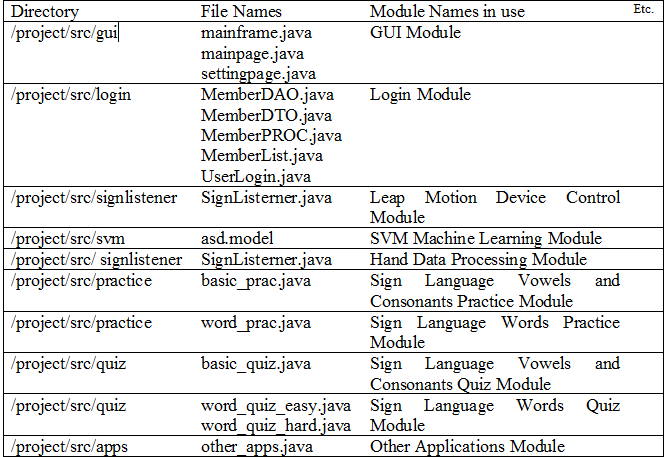
\includegraphics[width=0.5\textwidth]{capture.png}
\caption{}
\end{figure}

\subsubsection{GUI Module\\}

KASLE has GUI environment. All the GUI stuffs are managed by this module. All other features operated by all other modules are operated based on GUI module. GUI module starts and controls overall process of program.
\\Class : class mainframe, class mainpage, class basic\_prac, class word\_prac, class basic\_quiz, class word\_quizeasy, class word\_quizhard, class setting\_page
\begin{figure}[H]
\centering
\includegraphics[width=0.5\textwidth]{mainpage.png}
{\caption*{Picture of mainpage}}
\end{figure}
\subsubsection{Login Module\\}

KASLE has 2 modes, login user mode and visitor mode. If user wants register id, user can register id from program site. User can login to the program, user will get the statistics of quiz data. If current user doesn't log in, visitior mode is applied.
\\All other modules are operated based on the mode applided by login module
\\Class : class MemberDAO, class MemberDTO, class MemberPROC, class MemberList, class UserLogin

\begin{figure}[H]
\centering
\includegraphics[width=0.5\textwidth]{cap_login.png}
{\caption*{Picture of login}}
\end{figure}
\subsubsection{Leap Motion Device Control Module\\}

Leap Motion device shoots a video of hand (30 frames per seconds) and analyze this 2D picture and convert into data set that represents 3D hand status. These detailed analyzing and converting process is handled by Leap Motion device.
Current hand status is represented by various variables of various forms such as hand position (based on three dimensions), palm direction(represented in geometrical data), each fingers bending angle, distance from other fingers etc.
\\And Leap motion device control module delivers converted data set of 3D hand status to SVM machine learning module.
\\Class : class SignListener

\begin{figure}[H]
\centering
\includegraphics[width=0.5\textwidth]{cap_tutorial.png}
{\caption*{3D model of current hand}}
\end{figure}
\subsubsection{SVM machine learning module\\}

This module receives hand data samples from leap motion control module. (Each hand data sample represents hand data status of each moment.) By combining and analyzing plenty of samples (using SVM machine learning algorithm), delicately refined hand data set is generated. Developer can assign this well-defined hand data to corresponding sign language.
\\(without refining process of SVM algorithm, accuracy of recognition drops sharply.
\\Class : class SignListener

\begin{figure}[H]
\centering
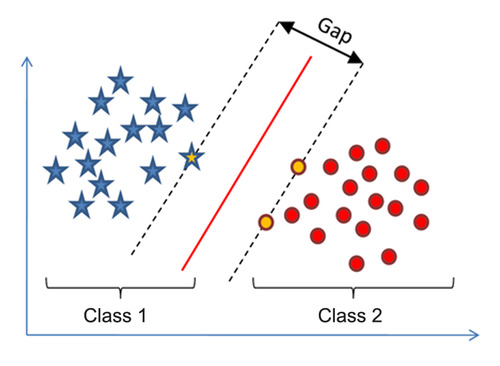
\includegraphics[width=0.5\textwidth]{SVM.jpg}
{\caption*{The graph of SVM}}
\end{figure}
\subsubsection{Hand data processing module\\}

This module receives information of current hand status from Leap Motion device control module and compares received data with data samples initially assigned to each sign language.
\\If there exists data sample corresponds to current received hand status data, this module recognizes input value as valid sign language and returns corresponding assigned sign language.
\\Class : class SignListener
\\There is no picture for this module.

\subsubsection{Sign language (vowels and consonants) practice module\\}

This module implements sign language vowel and consonant practice. It shows question and answer for each question. They consist of vowels and consonants. User can follow shown sign language. This module compares user’s hand status with answer for current question. If they are same, it proceeds to next question and repeat above process until all the practice is over.
\\Class : class basic\_prac
\begin{figure}[H]
\centering
\includegraphics[width=0.5\textwidth]{cap_basic_prac.png}
{\caption*{The picture of basic practice}}
\end{figure}
\subsubsection{ Sign language (words) practice module\\}
This module implements sign language words practice. It shows question and answer for each question. They consist of words. User can follow shown sign language.  This module compares user’s hand status with answer for current question. If they are same, it proceeds to next question and repeat above process until all the practice is over.
\\Class : class word\_prac
\begin{figure}[H]
\centering
\includegraphics[width=0.5\textwidth]{cap_word_prac.png}
{\caption*{The picture of basic practice}}
\end{figure}
\subsubsection{Sign language (words) game module\\}
This module implements sign language game. It shows question in forms of rain. Also shows user’s score on the right. (indicates how well user answers for given questions.) Questions consist of words. This module receive user’s hand status and compares it with an answer for current question. After 1 minute , this module reflects the result of comparison to score and game is over.
\\Class : , class rain\_game
\begin{figure}[H]
\centering
\includegraphics[width=0.5\textwidth]{cap_rain_game.png}
{\caption*{The picture of rain game}}
\end{figure}



\subsection{Use Cases\\} 
\subsubsection{Sign-in and Login\\}
This use case satisfies ‘user can login’ and ‘Separating user mode by normal user and visitor.’ requirements.
\\Step 1.
\\Run KASLE program
\\Step 2.
\\Click ‘회원가입’(Sign-in) button.
\\Step 3.
\\Enter the basic information of user.
\\Step 4. 
\\Click ‘확인’(OK) button.
\\Step 5.
\\Click ‘로그인’ (login) button.
\\Step 6.
\\Enter ID and password.
\\Step 7.
\\Check whether there is error message or not.

\subsubsection{User can see his(her) own historical information\\}
This use case satisfies ‘User can see his(or her) accumulated historical information on KASLE program.’ requirement.
\\Step 1.
\\Run KASLE program
\\Step 2.
\\Click Login button.
\\Step 3. 
\\Enter ID and password. (login is necessarily needed.)
\\Step 4.
\\After you are logged in, click ‘개인기록’(personal history) at the main menu.
\\Step 5. 
\\Check your accumulated information on KASLE program. (average of game scores until then, how many practices you’ve ever done, etc.)



\subsubsection{Properly showing hand data\\} 
This use case satisfies ‘Get hand data Using LeapMotion hardware’ requirement.
\\Step 1.
\\Run KASLE program
\\Step 2.
\\Login (it is not necessarily needed.)
\\Step 3.
\\Click any practice or game menu at main page.
\\Step 4. 
\\Check the box at the bottom side of screen which represents user’s current hand status.



\subsubsection{Run Vowels and Consonants Practice\\}
This use case satisfies ‘User can practice vowels and consonants of sign language’ requirement.
\\Step 1.
\\Run KASLE program
\\Step 2.
\\Login (it is not necessarily needed.)
\\Step 3.
\\Click ‘자모음연습’ button at main menu.
\\Step 4. 
\\Set the mode (vowels only, consonants only, both)
\\Step 5.
\\Check the box at the top of screen which shows current question.
\\Step 6.
\\Check the box at the right bottom side of screen which represents answer of current question.
\\Step 7.
\\Check the box at the top of screen which shows current question.
\\Step 8.
\\Check the box at the left bottom side of screen which represents user’s current hand status.
\\Step 9. 
\\Follow the answer and check whether current question is finished and next question is shown.
\\Step 10.
\\Check all the questions are shown.

\subsubsection{ Run Words Practice\\}
This use case satisfies ‘User can practice words of sign language’ requirement.
\\Step 1.
\\Run KASLE program
\\Step 2.
\\Login (it is not necessarily needed.)
\\Step 3.
\\Click ‘낱말연습’ button at main menu.
\\Step 4. 
\\Check the box at the top of screen which shows current question.
\\Step 5. 
\\Check the box at the right bottom side of screen which represents answer of current question.
\\Step 6.
\\Check the box at the top of screen which shows current question.
\\Step 7.
\\Check the box at the left bottom side of screen which represents user’s current hand status.
\\Step 8. 
\\Follow the answer and check whether current question is finished and next question is shown.
\\Step 9.
\\Check all the questions are shown.

\subsubsection{Run Words Practice\\}

This use case satisfies ‘User can practice words of sign language’ requirement.
\\Step 1.
\\Run KASLE program
\\Step 2.
\\Login (it is not necessarily needed.)
\\Step 3.
\\Click ‘낱말연습’ button at main menu.
\\Step 4. 
\\Check the box at the top of screen which shows current question.
\\Step 5.
\\Check the box at the right bottom side of screen which represents answer of current question.
\\Step 6.
\\Check the box at the top of screen which shows current question.
\\Step 7.
\\Check the box at the left bottom side of screen which represents user’s current hand status.
\\Step 8. 
\\Follow the answer and check whether current question is finished and next question is shown.
\\Step 9.
\\Check all the questions are shown.

\subsubsection{Run Vowels and Consonants Quiz\\}
This use case satisfies ‘User can play game on vowels and consonants.
\\Step 1.
\\Run KASLE program
\\Step 2.
\\Login (it is not necessarily needed.)
\\Step 3.
\\Click ‘자모음게임’ button at main menu.
\\Step 4. 
\\Set the mode (vowels only, consonants only, both)
\\Step 5.
\\Check the box at the top of screen which shows current question.
\\Step 6.
\\Check the box at the top of screen which shows current question.
\\Step 7.
\\Check the box at the bottom side of screen which represents user’s current hand status.
\\Step 8. 
\\If answering time (5 seconds per question) is over, program must finishes current question and shows next question.
\\Step 9.
\\ Check whether the result of questions is properly reflected to score.
\\Step 10.
\\ Check all the questions are shown.

\subsubsection{Run Words Quiz\\}
This use case satisfies ‘User can play game on words.
\\Step 1.
\\Run KASLE program
\\Step 2.
\\Login (it is not necessarily needed.)
\\Step 3.
\\Click ‘낱말게임’ button at main menu.
\\Step 4.
\\Check the box at the top of screen which shows current question.
\\Step 5.
\\Check the box at the top of screen which shows current question.
\\Step 6.
\\Check the box at the bottom side of screen which represents user’s current hand status.
\\Step 7. 
I\\f answering time (5 seconds per question) is over, program must finishes current question and shows next question.
\\Step 8.
\\Check whether the result of questions is properly reflected to score.
\\Step 9.
\\Check all the questions are shown.

\subsubsection{Share to other applications\\}
This use case satisfies ‘Posting text entered by hand movement to Social Network Service’ requirement.
\\Step 1.
\\Run KASLE program
\\Step 2.
\\Login (it is not necessarily needed.)
\\Step 3.
\\Click ‘공유하기’(share) button at main menu.
\\Step 4. 
\\Check the box at the bottom of screen which shows your hand data.
\\Step 5.
\\Express any words in sign language.
\\Step 6.
\\Check the box at the top of screen which shows words which is described by sign language.
\\Step 7.
\\If you want to express things that can’t be described by sign language, you can click button on the screen to help you. Check whether buttons are operating properly.
\\Step 8. 
\\Choose the application to which you want to share your text written by KASLE.
\\Step 9.
\\Click ‘공유하기’(share) button. 
\\Step 10.
\\Check whether there is no error message.
\\Step 11. 
\\Check the external application of your choice to receive text written by KASLE properly.
\\\\\\
\ifCLASSOPTIONcompsoc
\IEEEraisesectionheading{\section{Software Installation Guide}\label{sec:Software Installation Guide}}
\else
\section{Software Installation Guide}
\label{sec:Software Installation Guide}
\fi
\subsection{Installation}
\subsubsection{System Requirement}
The minimum system requirements are:\\
1. Windows® 7+ or Mac® OS X 10.7+\\
2. AMD Phenom™ II or Intel® Core™ i3/i5/i7 processor\\
3. 2 GB RAM\\
4. USB 2.0 port\\
5. Internet connection\\
6. Java 
\subsubsection{Installation for LeapMotion Driver}
1. Turn on your Computer. If it doesn't turn on, please contact your adminstrator.\\
2. Double click on the your favorite browser, as chrome, explorer, or firefox.\\ 

\begin{figure}[H]
\centering
\includegraphics[width=0.5\textwidth]{Internet.png}
{\caption*{internet browser looks like this}}
\end{figure}
3. If you can't turn on the internet, please check your connections.\\ 
\begin{figure}[H]
\centering
\includegraphics[width=0.3\textwidth]{Connection.png}
{\caption*{If it is red or exclamination mark
		  please contact adminstaror }}
\end{figure}

4. Next, insert https://www.leapmotion.com/setup  on the browser\\
\begin{figure}[H]
\centering
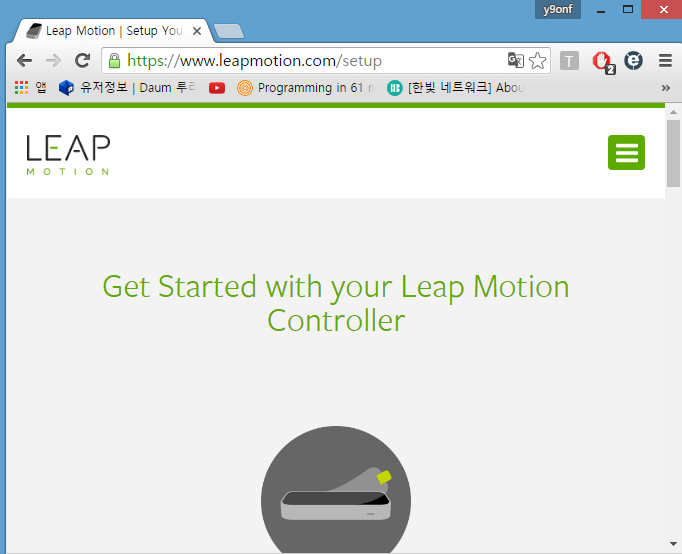
\includegraphics[width=0.3\textwidth]{address.png}
{\caption*{Location address}}
\end{figure}

5. Then, on the website, please click on the 'Windows Download(DESKTOP)'\\
\begin{figure}[H]
\centering

\includegraphics[width=0.3\textwidth]{Download.png}
{\caption*{Please click  this button twice }}
\end{figure}

6. When the driver finished download, please click on the driver, and click execute\
7.Check your security control and allow program to download
\begin{figure}[H]
\centering
\includegraphics[width=0.3\textwidth]{Download1.png}
{\caption*{Please click execute}}
\end{figure}

8.If you see download is completed, check 'experience LeapMotion'and click finish \\
\begin{figure}[H]
\centering
\includegraphics[width=0.3\textwidth]{Download3.png}
{\caption*{Please click finish}}
\end{figure}

9.You will see main page of LeapMotion applications.
\begin{figure}[H]
\centering
\includegraphics[width=0.3\textwidth]{Download4.png}
{\caption*{If you see this picture, your download is completed }}
\end{figure}

NOTE: If software doesn't work, or if you have any other questions \\
Please contact our email, kyoon3@naver.com\\
\subsubsection{Installation for KASLE}
1. Turn on your Computer. If it doesn't turn on, please contact your adminstrator.\\
2. Double click on the your favorite browser, as chrome, explorer, or firefox.\\ 

\begin{figure}[H]
\centering
\includegraphics[width=0.5\textwidth]{Internet.png}
{\caption*{internet browser looks like this}}
\end{figure}

3. If you can't turn on the internet, please check your connections.\\ 

\begin{figure}[H]
\centering
\includegraphics[width=0.3\textwidth]{Connection.png}
{\caption*{If it is red or exclamination mark
		  please contact adminstaror }}
\end{figure}

4. Next, insert https://github.com/hoiek12/java-KASLE\\

\begin{figure}[H]
\centering
\includegraphics[width=0.3\textwidth]{Download5.png}
{\caption*{I }}
\end{figure}
5. Then, on the repository section, please click download ZIP. Download will begin shortly.\\

\begin{figure}[H]
\centering
\includegraphics[width=0.3\textwidth]{Download6.png}
{\caption*{Click download ZIP }}
\end{figure}
6. When the KASLE finished download, please click finish\\
7. Go to the downloaded folder and double click on KASLE.exe. \\
8. If KASLE.exe works, close your browser and enjoy KASLE.\\
\begin{figure}[H]
\centering
\includegraphics[width=0.3\textwidth]{mainpage.png}
{\caption*{Enjoy }}
\end{figure}
NOTE: If software doesn't work, or if you have any other questions \\
Please contact our email, kyoon3@naver.com\\
\\\\\\
\ifCLASSOPTIONcompsoc
\IEEEraisesectionheading{\section{Discussion}\label{sec:Discussion}}
\else
\section{Discussion}
\label{sec:Discussion}
\fi
\subsection{Discussion\\}
This software development project was first time for all of our team members. So, we expected that our project could encounter a lot of adversities. And it was actually tough more than we expected. And there were so many unexpected challenges we’ve met. But of course, we have learned a lot of things from that challenges. We could understand how the software development process goes and how many problems that could possibly happen during the process.

At the very beginning of the project, we had problem to decide our program to develop. There were so many ideas. So negotiation was not that easy. After we decide what to develop, there were many problems we had to handle. So, we tried to meet as frequent as possible. However, we could not avoid communication problem. When our team members had meeting, we drew blue print of program and decide who has responsible for what. But we could not decide every implementation details and design. So, we had to contact each other to negotiate and how to achieve each member's job and how to integrate each member's code. 

Second hardship was using open source algorithms. At first, we thought that using open source code must be easy. Because we thought that if we need some feature and there is a open source code which implements our feature, we can just copy and paste it to our code. But if we do that so, there were so many errors. We had to modify source code to make it work together smoothly with other features.

Third hardship was related to hardware issue. We used hardware called LeapMotion to get data from hands. However leap motion camera was not good as we thought, so it was very hard to get accurate data. So, we had to apply SVM machine learning algorithm to improve accuracy. Using SVM algorithm was also big challenge for us.

Forth, we had an problem with Java. Not because of Java itself, but the problem was our low experience with java. So, we had to study how JAVA works.

Lastly, we didn’t have experiences working together with other people on one project. And making one function was kind of easy but integrating them and make them work together was harder than we thought.
Also, there were valuable experiences despite these hardships.

First was we could learn Java. We didn’t have any experience with Java before this project. For now, we have learned a lot of things about JAVA and software development.
Second, implementing small feature was relatively easy. However integrating them and make it work together without error was extremely hard. It requires not only coding each feature properly but also proper structure of program.
Third, we learned how to make GUI. Before this project we thought that making GUI was easy. But in reality, it was not that easy to implement detailed implementation. So, we use a lot of tools to help us like 'Jigloo' and 'Swing-Worker'.
\clearpage
\begin{figure}[H]
\includegraphics[width=0.9\textwidth]{My.png}
\caption{}
\end{figure}















% An example of a floating figure using the graphicx package.
% Note that \label must occur AFTER (or within) \caption.
% For figures, \caption should occur after the \includegraphics.
% Note that IEEEtran v1.7 and later has special internal code that

% is designed to preserve the operation of \label within \caption
% even when the captionsoff option is in effect. However, because
% of issues like this, it may be the safest practice to put all your
% \label just after \caption rather than within \caption{}.
%
% Reminder: the "draftcls" or "draftclsnofoot", not "draft", class
% option should be used if it is desired that the figures are to be
% displayed while in draft mode.
%
%\begin{figure}[!t]
%\centering
%\includegraphics[width=2.5in]{myfigure}
% where an .eps filename suffix will be assumed under latex, 
% and a .pdf suffix will be assumed for pdflatex; or what has been declared
% via \DeclareGraphicsExtensions.
%\caption{Simulation results for the network.}
%\label{fig_sim}
%\end{figure}

% Note that the IEEE typically puts floats only at the top, even when this
% results in a large percentage of a column being occupied by floats.
% However, the Computer Society has been known to put floats at the bottom.


% An example of a double column floating figure using two subfigures.
% (The subfig.sty package must be loaded for this to work.)
% The subfigure \label commands are set within each subfloat command,
% and the \label for the overall figure must come after \caption.
% \hfil is used as a separator to get equal spacing.
% Watch out that the combined width of all the subfigures on a 
% line do not exceed the text width or a line break will occur.
%
%\begin{figure*}[!t]
%\centering
%\subfloat[Case I]{\includegraphics[width=2.5in]{box}%
%\label{fig_first_case}}
%\hfil
%\subfloat[Case II]{\includegraphics[width=2.5in]{box}%
%\label{fig_second_case}}
%\caption{Simulation results for the network.}
%\label{fig_sim}
%\end{figure*}
%
% Note that often IEEE papers with subfigures do not employ subfigure
% captions (using the optional argument to \subfloat[]), but instead will
% reference/describe all of them (a), (b), etc., within the main caption.
% Be aware that for subfig.sty to generate the (a), (b), etc., subfigure
% labels, the optional argument to \subfloat must be present. If a
% subcaption is not desired, just leave its contents blank,
% e.g., \subfloat[].


% An example of a floating table. Note that, for IEEE style tables, the
% \caption command should come BEFORE the table and, given that table
% captions serve much like titles, are usually capitalized except for words
% such as a, an, and, as, at, but, by, for, in, nor, of, on, or, the, to
% and up, which are usually not capitalized unless they are the first or
% last word of the caption. Table text will default to \footnotesize as
% the IEEE normally uses this smaller font for tables.
% The \label must come after \caption as always.
%
%\begin{table}[!t]
%% increase table row spacing, adjust to taste
%\renewcommand{\arraystretch}{1.3}
% if using array.sty, it might be a good idea to tweak the value of
% \extrarowheight as needed to properly center the text within the cells
%\caption{An Example of a Table}
%\label{table_example}
%\centering
%% Some packages, such as MDW tools, offer better commands for making tables
%% than the plain LaTeX2e tabular which is used here.
%\begin{tabular}{|c||c|}
%\hline
%One & Two\\
%\hline
%Three & Four\\
%\hline
%\end{tabular}
%\end{table}


% Note that the IEEE does not put floats in the very first column
% - or typically anywhere on the first page for that matter. Also,
% in-text middle ("here") positioning is typically not used, but it
% is allowed and encouraged for Computer Society conferences (but
% not Computer Society journals). Most IEEE journals/conferences use
% top floats exclusively. 
% Note that, LaTeX2e, unlike IEEE journals/conferences, places
% footnotes above bottom floats. This can be corrected via the
% \fnbelowfloat command of the stfloats package.







% if have a single appendix:
%\appendix[Proof of the Zonklar Equations]
% or
%\appendix  % for no appendix heading
% do not use \section anymore after \appendix, only \section*
% is possibly needed

% use appendices with more than one appendix
% then use \section to start each appendix
% you must declare a \section before using any
% \subsection or using \label (\appendices by itself
% starts a section numbered zero.)
%




% you can choose not to have a title for an appendix
% if you want by leaving the argument blank



% trigger a \newpage just before the given reference
% number - used to balance the columns on the last page
% adjust value as needed - may need to be readjusted if
% the document is modified later
%\IEEEtriggeratref{8}
% The "triggered" command can be changed if desired:
%\IEEEtriggercmd{\enlargethispage{-5in}}

% references section

% can use a bibliography generated by BibTeX as a .bbl file
% BibTeX documentation can be easily obtained at:
% http://mirror.ctan.org/biblio/bibtex/contrib/doc/
% The IEEEtran BibTeX style support page is at:
% http://www.michaelshell.org/tex/ieeetran/bibtex/
%\bibliographystyle{IEEEtran}
% argument is your BibTeX string definitions and bibliography database(s)
%\bibliography{IEEEabrv,../bib/paper}
%
% <OR> manually copy in the resultant .bbl file
% set second argument of \begin to the number of references
% (used to reserve space for the reference number labels box)


% biography section
% 
% If you have an EPS/PDF photo (graphicx package needed) extra braces are
% needed around the contents of the optional argument to biography to prevent
% the LaTeX parser from getting confused when it sees the complicated
% \includegraphics command within an optional argument. (You could create
% your own custom macro containing the \includegraphics command to make things
% simpler here.)
%\begin{IEEEbiography}[{\includegraphics[width=1in,height=1.25in,clip,keepaspectratio]{mshell}}]{Michael Shell}
% or if you just want to reserve a space for a photo:


% if you will not have a photo at all:

% insert where needed to balance the two columns on the last page with
% biographies
%\newpage


% You can push biographies down or up by placing
% a \vfill before or after them. The appropriate
% use of \vfill depends on what kind of text is
% on the last page and whether or not the columns
% are being equalized.

%\vfill

% Can be used to pull up biographies so that the bottom of the last one
% is flush with the other column.
%\enlargethispage{-5in}



% that's all folks
\end{document}


